%% Public domain image from
%% http://www.public-domain-image.com/objects/computer-chips/slides/six-computers-chips-circuits.html
\renewcommand\chapterillustration{OGL_intro/chapterImage}



\chapter{컴퓨터 그래픽스 소개}

컴퓨터 그래픽스(computer graphics)란 ‘컴퓨터를 이용한 그래픽스’이다. 그래픽스는 그리기, 쓰기 등을 의미하는 그리스어  ‘$\gamma\rho\alpha\varphi\acute{\eta}$(graph\'{e})’를 어원으로 하며, 어떠한 표면에 시각적인 표현을 드러내는 것이다. 다시 말해, 컴퓨터 그래픽스라는 것은 컴퓨터를 활용하여 시각적으로 관찰할 수 있는 영상을 생성하는 것이다.
그래픽스는 단순히 시각 정보 그 자체를 의미하는 것이 아니라, 이러한 시각 정보를 생성하는 것과 관련된 다양한 이론과 기술을 다루는 분야이다.
이 장에서는 컴퓨터 그래픽스가 무엇인지를 살펴보고 그 응용 분야를 알아볼 것이다.
\index{$\gamma\rho\alpha\varphi\acute{\eta}$}\index{컴퓨터 그래픽스}\index{computer graphics}

\section{컴퓨터 그래픽스의 의미}

사실 컴퓨터 그래픽스는 매우 넓은 의미를 가지며, 컴퓨터를 이용하여 텍스트(text)나 음향를 생성하는 것을 제외하고는 거의 모든 것이 그래픽스의 범주에 들어간다는 이야기까지 있다. 위키피디아(wikipedia)에 예시된 몇 가지 컴퓨터 그래픽스 용어의 활용예를 보면 다음과 같다 \cite{wiki:computerGraphics}.

\begin{itemize}
\item 컴퓨터를 이용한 영상 데이터의 표현과 조작
\item 영상을 생성하고 조작하기 위한 다양한 기술
\item 시각적 콘텐츠를 디지털 기술로 합성/조작하는 방법을 연구하는 전산학 분야
\end{itemize}

3차원 컴퓨터 그래픽스라는 것은 이러한 그래픽스 가운데 3차원 기하(geometry) 객체 표현을 사용하는 그래픽스 분야이다. 컴퓨터 게임이나 영화의 경우 결과 영상은 2차원 공간인 모니터나 스크린에 표현되지만, 이 영상을 얻기 위해 처리되는 데이터는 3차원 공간에서 정의되고 조작되므로 3차원 컴퓨터 그래픽스라고 부른다.
컴퓨터 그래픽스의 세부 분야는 모델링(modeling), 애니메이션(animation), 렌더링(rendering)으로 크게 구분이 된다.
\index{모델링}\index{애니메이션}\index{렌더링}


컴퓨터 그래픽스에서 모델링(modeling)은 영상 생성에 사용되는 객체의 기하적 특성을 정의하는 일이라고 할 수 있다. 객체를 표현하기 위해 사용되는 정점의 수를 결정하고, 이 정점들의 위치와 연결성을 설정하고, 그려질 면을 구성하는 일 등이 이 분야에 포함된다.

컴퓨터 그래픽스에서 사용되는 애니메이션(animation)은 모델링 과정을 통해 결정된 기하객체에 대해 시간에 따른 변화를 설정하는 작업이다. 일반적으로 이 변화의 대상은 기하객체의 위치가 되어, 시간이 흐름에 따라 객체가 움직이는 모습을 보이게 된다. 그러나 위치만이 애니메이션의 유일한 대상은 아니며, 시간에 따라 색상이 변하든가 물체에 적용된 텍스처(texture)가 변하는 등의 일도 모두 애니메이션의 범주에 든다.

렌더링(rendering)을 모델링된 기하객체를 최종 관찰 표면에 그려내어 영상을 생성하는 분야이다. 이를 위해서 조명 모델을 이용하여 표면의 색상 및 밝기 등을 결정하고, 이렇게 결정된 색상을 2차원의 공간으로 투영하여 영상을 생성하는 것이다.


\section{컴퓨터 그래픽스의 응용 분야}

컴퓨터 그래픽스는 게임이나 영화를 포함하여 다양한 영역에서 사용된다. 게임이나 영화는 컴퓨터 그래픽스가 엔터테인먼트를 위해 사용되는 대표적인 영역이며, 이 밖에도 다양한 과학기술 분야 및 산업 영역에서 컴퓨터 그래픽스가 활용되고 있다. 이런 분야의 예로는 정보 가시화, 설계, 시뮬레이션 등이 있다. 이 절에서는 이런 분야에 사용된 컴퓨터 그래픽스 기술의 예를 살펴볼 것이다. 이러한 예를 통해 컴퓨터 그래픽스에서 어떠한 문제들을 다루는지에 대한 대략적인 이해를 할 수 있을 것이다.



\subsubsection{캐드(CAD) 분야}

\index{CAD}\index{캐드}
캐드는 컴퓨터를 활용한 설계, 즉 ‘Computer-Aided Design’의 머릿글자를 따서 만든 단어로 건축, 제조 등 다양한 분야의 설계를 컴퓨터 그래픽스 기술을 활용하여 수행하는 분야이다. 이 캐드 기술 덕분에 설계에 필요한 인력, 시간, 노력 등을 대폭 줄일 수 있게 되었으며 업무 효율과 생산성이 높아졌다. 이런 캐드 기술은 제조 공정에 컴퓨터가 활용되는 컴퓨터 기반 제조(Computer-Aided Manufacturing) 기술로 발전하여 수치 제어 기계를 통해 높은 효율과 정밀도를 가진 제품 생산 기술로 이어진다. 그림 \ref{fig:OGL_intro:CAD}는 이러한 CAD 분야에 적용된 그래픽스 기술의 예이다.

\begin{figure}[h!]
  \centering
    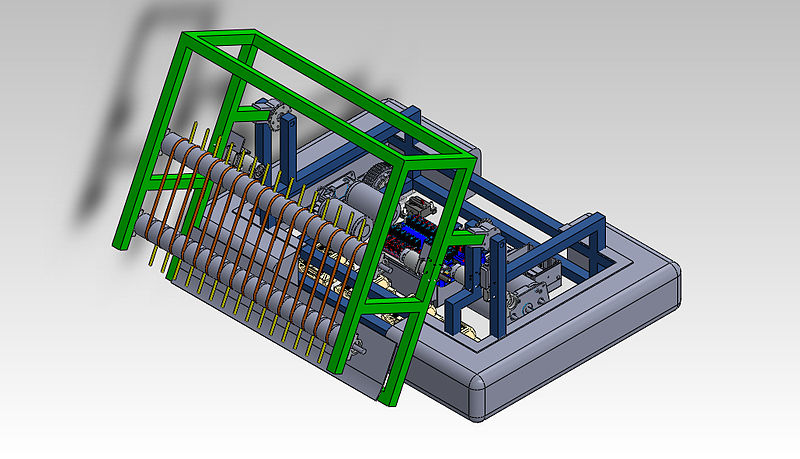
\includegraphics[width=11cm]{OGL_intro/CAD.jpg}
    \caption{CAD에 활용된 그래픽스 기술의 예}
    \label{fig:OGL_intro:CAD}
\end{figure}


\subsubsection{가상 현실(virtual reality)}

\index{virtual reality}\index{가상 현실}
가상이라는 말은 ‘버추얼(virtual)’이라는 단어를 번역한 것인데, 가상이라는 단어는 ‘실물이 아닌’ 것이라는 느낌이 강하지만, ‘버추얼’이라는 단어는 ‘사실과 거의 차이가 없는’ 것의 의미가 더 강하다. 따라서 가상현실은 가짜 세계가 아니라 실세계와 구분하기 힘든 세계를 재현하는 것이 목표이다. 따라서 가상현실 기술은 “존재하지 않는 가상의 환경을 표현하되 마치 실재하는 것처럼 느껴지도록 만드는 기술”이라 할 수 있다.

\index{HMD}\index{head mounted display}\index{data glove}\index{데이터 장갑}
가상현실을 가능하게 하는 기술적 요소는 입체화면, 3차원 입체 음향, 데이터 장갑 등의 입출력 장비,  컴퓨터 그래픽스 등이 있다.  또한 실재감을 제공하기 위해 인지과학, 전자공학, 기계공학 등의 다양한 분야의 연구결과들이 활용된다. 그림 \ref{fig:OGL_intro:VRHMD}는 이러한 가상현실 분야에 적용된 그래픽스 기술의 결과를 시각적으로 제공하기 위해 머리에 쓰고 보는 장치(HMD, head-mounted display)와 상호작용에 사용되는 데이터 장갑(data glove)의 예를 보이고 있다.

\begin{figure}[h!]
  \centering
    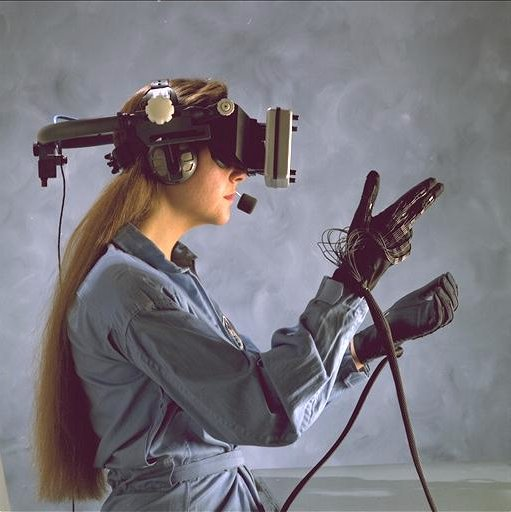
\includegraphics[width=13cm]{OGL_intro/virtualRealityHMD.jpg}
    \caption{가상현실 콘텐츠와 상호작용하기 위한 장비}
    \label{fig:OGL_intro:VRHMD}
\end{figure}

\subsubsection{실사 수준 고품질 가시화 (photorealistic visualization)}

\index{photorealistic rendering}\index{실사 수준 렌더링}
컴퓨터 그래픽스의 수준이 높아지면서 가상 객체의 렌더링 결과를 실세계 물건과 구별하기가 매우 힘들어지고 있다. 이러한 고품질 렌더링 기술을 바탕으로 상품 등을 실제로 만들지 않고도 사용자가 시각적으로 확인할 수 있는 실사 수준의 고품질 가시화 기술이 다양한 산업 분야에 적용되고 있다. 그림 \ref{fig:OGL_intro:photorealistic}는 이러한 실사 수준의 가시화 기술을 적용하여 얻은 이미지의 예이다. 그림에서 확인할 수 있는 바와 같이 현대의 그래픽스 기술은 사진과 거의 구분할 수 없는 수준의 고품질 렌더링이 가능하다. 이러한 실사 수준의 가시화는 전통적으로 하나의 이미지를 얻는 데에 오랜 시간이 소요되므로, 실시간 그래픽스의 영역이 아니었다. 하지만, 최근의 하드웨어 성능 발전과 그래픽스 알고리즘의 발전으로 이러한 실사 수준의 렌더링이 머지 않아 실시간 가시화 시스템에도 실현될 것이다.

\begin{figure}[h!]
  \centering
    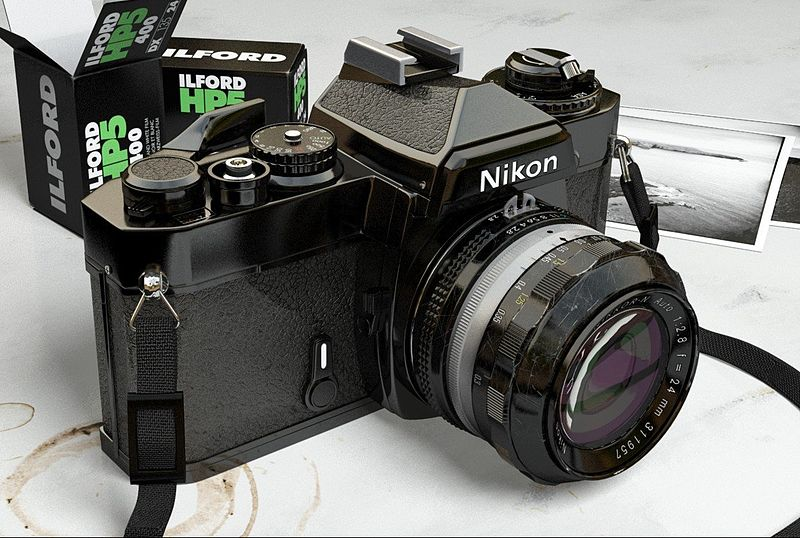
\includegraphics[width=9cm]{OGL_intro/photorealistic.jpg}
    \caption{실사 수준의 고품질 가시화 결과}
    \label{fig:OGL_intro:photorealistic}
\end{figure}

\subsubsection{컴퓨터 아트 (computer art)}

컴퓨터 그래픽스 기술은 예술적 창작물을 만드는 분야에도 다양하게 활용되고 있다. 그림 \ref{fig:OGL_intro:art}는 이러한 컴퓨터 아트 분야에 그래픽스 기술이 적용된 예를 보이고 있다. 

\begin{figure}[h!]
  \centering
    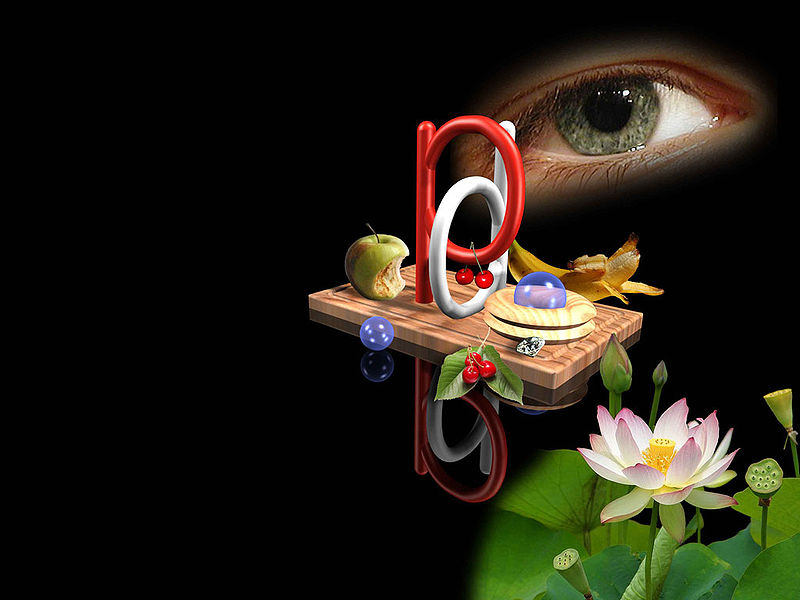
\includegraphics[width=9cm]{OGL_intro/computerArt.jpg}
    \caption{컴퓨터 그래픽스를 활용한 예술 작품의 예}
    \label{fig:OGL_intro:art}
\end{figure}

\subsubsection{컴퓨터 애니메이션(computer animation) 영화}

\index{컴퓨터 애니메이션 영화}\index{computer animation film}
컴퓨터 그래픽스가 활용되는 대표적인 산업 분야가 바로 컴퓨터 애니메이션 영화이다. 애니메이션 영화 산업에서 이제 컴퓨터 그래픽스는 가장 중요한 기술로 자리잡았다. 영화는 그 특성상 상호작용성(interactivity)이 요구되지 않기 때문에 실시간에 요구되는 영상을 생성해야할 필요는 없다. 따라서 이 분야에 적용되는 컴퓨터 그래픽스 기술은 오랜 시간 동안 렌더링 작업을 수행하여 한 장 한 장의 이미지를 매우 높은 수준의 품질로 생성한다. 이러한 렌더링 방식을 오프라인 렌더링(offline rendering)이라고 하며, 게임과 같은 분야에서 사용되는 실시간 렌더링(realtime rendering)과는 영상 생성의 과정이나 결과가 현격히 차이가 난다. 그림 \ref{fig:OGL_intro:animation}는 이러한 컴퓨터 애니메이션 작품의 예를 보이고 있다.


\begin{figure}[h!]
  \centering
    
\includegraphics[width=8cm]{OGL_intro/animation.jpg}
    \caption{BYU 애니메이션의 "파자마 글래디에터(Pajama Gladiator)"에 나오는 괴물 캐릭터}
    \label{fig:OGL_intro:animation}
\end{figure}

\begin{figure}[h!]
  \centering
    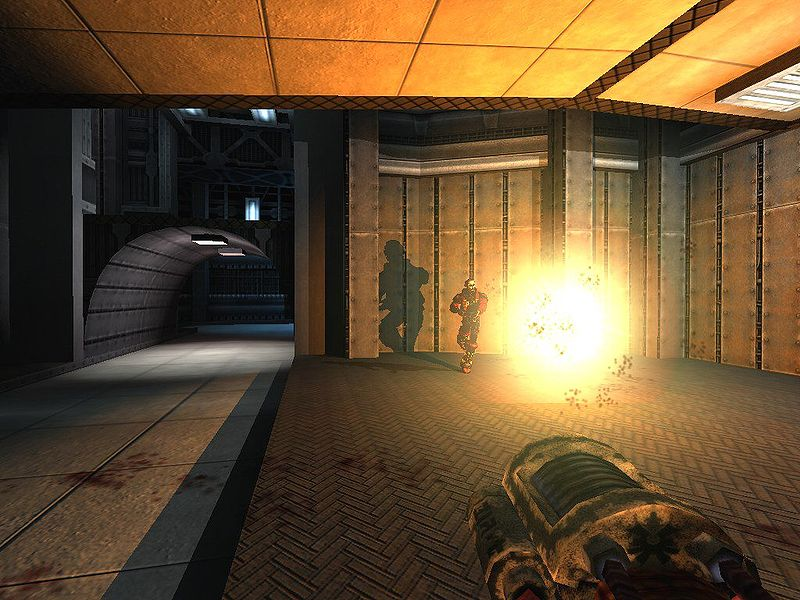
\includegraphics[width=8cm]{OGL_intro/game.jpg}
    \caption{그래픽 기술을 활용한 컴퓨터 게임의 예}
    \label{fig:OGL_intro:game}
\end{figure}

\subsubsection{컴퓨터 게임(computer game)}

\index{computer game}\index{컴퓨터 게임}
컴퓨터 그래픽스가 가장 상업적으로 성공한 분야 중에 하나이다. 컴퓨터 애니메이션과 달리 상호작용성(interactivity)가 매우 중요하며, 그 결과 초당 30 여 장의 영상을 즉각적으로 생성해낼 수 있는 실시간 고속 렌더링 기술이 매우 중요하다. 이러한 실시간 렌더링 기술은 오프라인 렌더링과 달리 GPU(graphics processing unit)가 장착된 고속 그래픽 장치에 최적화된 렌더링 기술이 사용된다. 

게임 산업의 발전은 이러한 그래픽 장치의 성능을 급격히 향상시켰으며, GPU 역시 CPU 처럼 사용자가 프로그램 가능한 상태로 발전하였다. 이에 따라 GPU의 병렬성을 활용하여 그래픽스 이외의 연산 작업을 수행하는 데에 그래픽스 장치를 활용하기도 한다. 컴퓨터 게임에 활용되는 실시간 렌더링 기술은 고품질의 영상을 빠른 시간에 그려내기 위한 다양한 기법을 발전시켰다. 이러한 기법의 예로는 렌더링 대상을 효과적으로 추려내기(culling), 텍스처의 활용, 법선벡터 조작 등을 통한 표면 질감 제어 등이 있다. 그림 \ref{fig:OGL_intro:game}는 이러한 컴퓨터 그래픽스 기술을 적용한 게임의 예이다.



\subsubsection{교육 및 훈련 (Training)}

‘백 번 보는 것보다 한 번 보는 게 낫다’고 하였다. 교육과 훈련에서도 책이나 다른  인쇄물을 통해 공부하는 것은 습득에 한계가 있다. 컴퓨터 그래픽스가 제공하는 강력한 가시화 기능은 교육과 훈련 분야에서 매우 효과적이다. 또한 실제 환경에서 훈련하기 힘든 전투나, 항공기 조종 등과 같은 분야의 훈련에서도 컴퓨터 그래픽스 기술을 활용한 모의 훈련이 매우 강력한 효과를 발휘한다. 특히 이러한 모의 훈련은 실제 훈련이 위험하거나 비용이 많이 드는 군사 분야 등에서 활용도가 높다. 그림 \ref{fig:OGL_intro:virtualTraining}은 미 공군과 해군에서 사용하고 있는 모의 훈련 시스템의 활용 장면이다.

\begin{figure}[h!]
  \centering
    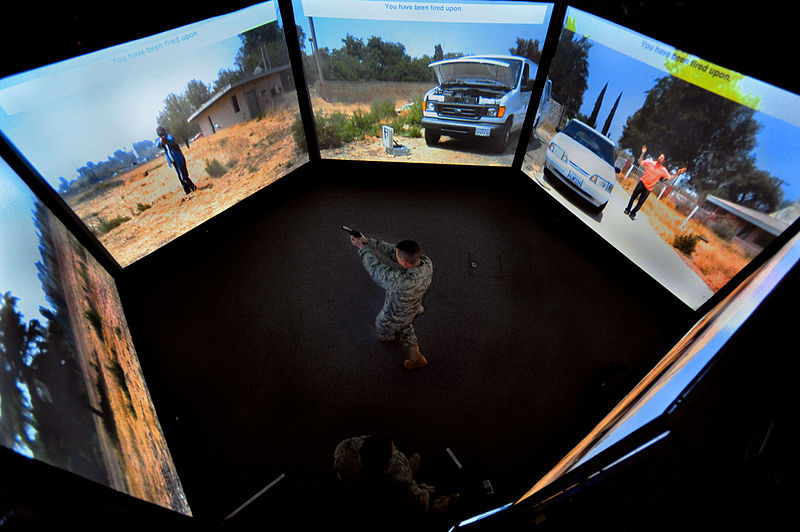
\includegraphics[height=4cm]{OGL_intro/virtualTraining.jpg}
    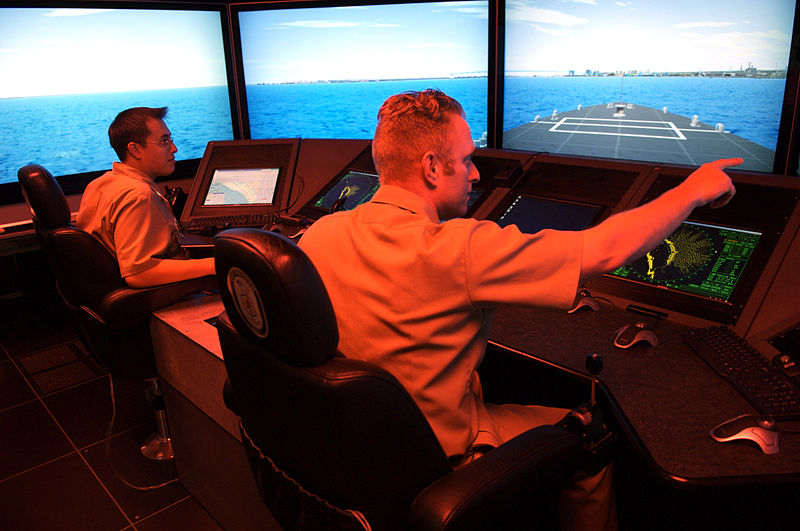
\includegraphics[height=4cm]{OGL_intro/virtualTraining2.jpg}
    \caption{미 공군과 해군의 가상 훈련}
    \label{fig:OGL_intro:virtualTraining}
\end{figure}


\subsubsection{정보 가시화 (information visualization)}

과학기술 분야에서 획득된 데이터를 이해하기 쉬운 형태로 표현하기 위해서는 이를 시각적 정보로 가공할 필요가 있다. 이러한 분야를 정보 가시화라고 하며, 자연 현상을 관찰하여 수집된 데이터를 활용하여 눈으로 확인할 수 있게 한다. 이런 가시화는 현상을 직관적으로 이해할 수 있게 하며, 패턴이나 추세 등을 파악하는 데에 큰 도움이 된다.
그림 \ref{fig:OGL_intro:visualization}은 초신성 폭발과 지형의 고도 데이터 등을 가시화한 예이다.


\begin{figure}[h!]
  \centering
    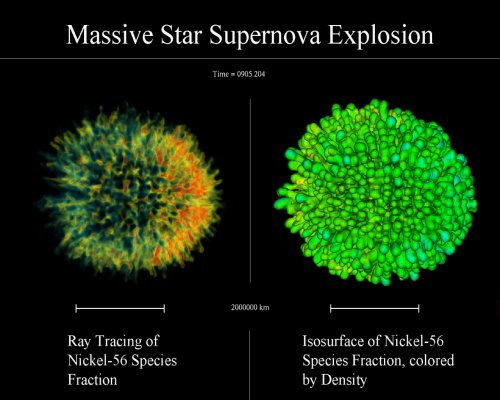
\includegraphics[height=6cm]{OGL_intro/visualization1.jpg}
    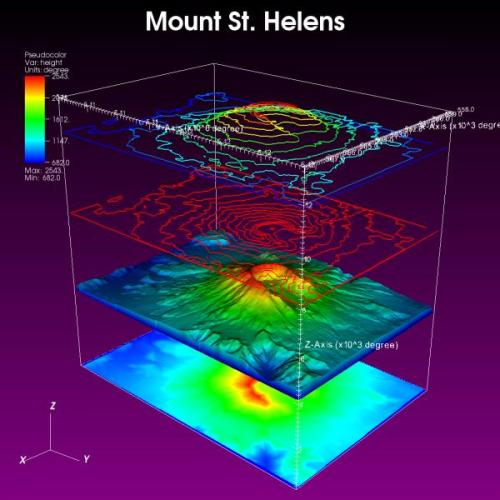
\includegraphics[height=6cm]{OGL_intro/visualization2.jpg}
    \caption{과학연구에 사용되는 데이터를 가시화한 예}
    \label{fig:OGL_intro:visualization}
\end{figure}

\section{컴퓨터 그래픽스의 간략한 역사}

이 절에서는 컴퓨터 그래픽스의 역사를 개략적으로 살펴본다. 시대별로 주요한 그래픽스 기술 발전을 살펴보겠다.

\subsubsection{1950 년대}

\index{테니스 포 투}\index{tennis for two}
컴퓨터 그래픽스가 시작된 시기이다. 컴퓨팅 역사의 초기이기도 하다. 간단한 선 그리기 등이 그래픽스의 주요 문제였다. 래스터 장치 보다는 벡터 디스플레이 장치를 이용한 그래픽 표현이 주를 이루었다. 벡터 디스플레이 장치는 전자총의 움직임을 따라 그림이 그려지게 되며, 화면을 화소로 구분하지 않는다. 그림 \ref{fig:OGL_intro:tennis4two}는 초창기 게임이라고 할 수 있는 `테니스 포 투(Tennis for Two)'의 시각적 결과를 보여주었던 벡터 디스플레이 시스템을 보이고 있다.

\begin{figure}[h!]
  \centering
    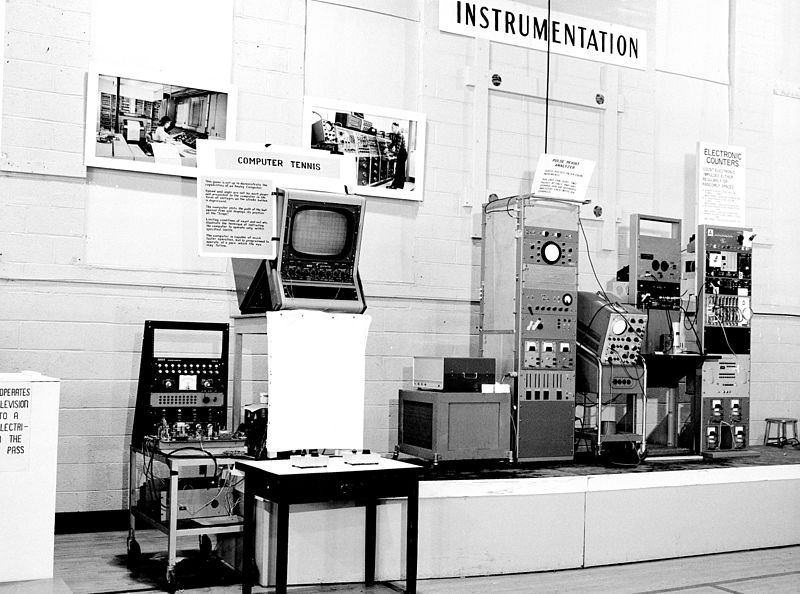
\includegraphics[height=6cm]{OGL_intro/tennis4two.jpg}
    \caption{초창기 게임인 `Tennis for Two'를 구동한 벡터 디스플레이 장치}
    \label{fig:OGL_intro:tennis4two}
\end{figure}

\subsubsection{1960년대}

\index{와이어 프레임}\index{wireframe}
60년대의 컴퓨터 그래픽스는 그림 \ref{fig:OGL_intro:wireframe}과 같이 객체의 연결구조만을 가시화하는 와이어 프레임(wireframe) 가시화 수준에 머물러 있었다. 다양한 그래픽 관련 기술과 산업이 나타나고, 후에 VR(virtual reality, 가상현실) 분야의 주요 장치가 되는 HMD(head mounted display) 장치도 이 무렵에 나오게 되었다. 

\begin{figure}[h!]
  \centering
    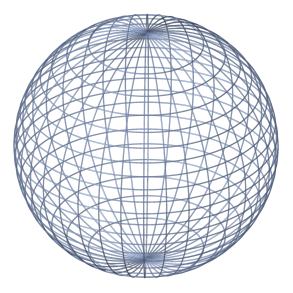
\includegraphics[height=6cm]{OGL_intro/wireframe.png}
    \caption{와이어프레임 가시화의 예}
    \label{fig:OGL_intro:wireframe}
\end{figure}

\subsubsection{1970 년대}

\index{raster graphics}\index{래스터 그래픽스}
래스터 그래픽스가 표준적인 그래픽스 표현 방식으로 자리를 잡게 된다.  래스터 그래픽스는 벡터 그래픽스와 달리 면을 칠하는 것이 더욱 쉬워지며, 면의 음영을 결정하거나, 화소별 색상을 계산하여 더욱 사실적인 고품질 이미지 생성이 가능하게 되었다. 와이어 프레임 표현이 아니라 면의 색상을 채워서 가시화하는 플랫 세이딩(flat shading)이 래스터 그래픽스 환경에서는 일반적으로 적용되게 된다. 그림 \ref{fig:OGL_intro:rastergraphics}는 화소의 개념과, 플랫 쉐이딩의 결과를 보이고 있다. 이 당시까지도 그래픽스 연구는 개인용 컴퓨터보다는 워크스테이션(workstation) 규모 이상에서 주로 이루어진다.

\begin{figure}[h!]
  \centering
    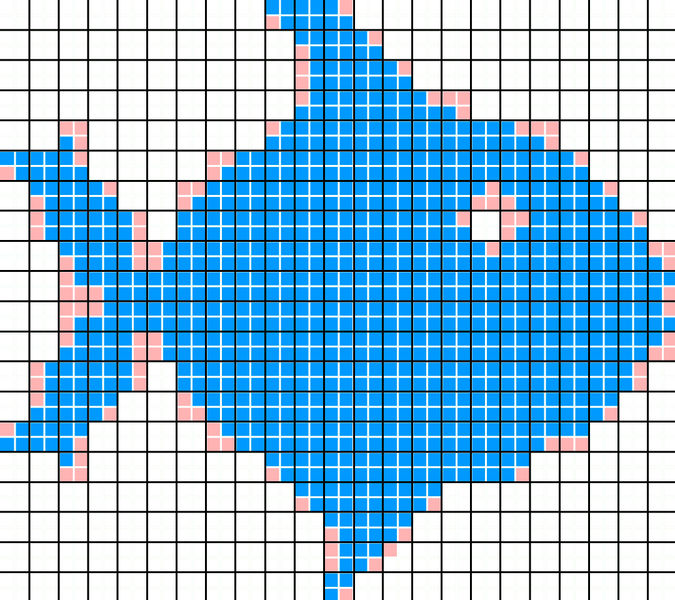
\includegraphics[height=4cm]{OGL_intro/rasterFish.jpg}
    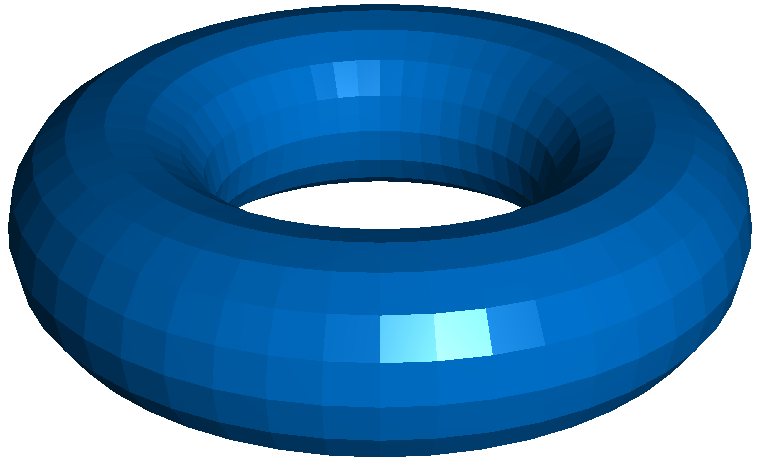
\includegraphics[height=4cm]{OGL_intro/flatShading.png}
    \caption{래스터 그래픽스의 기본 요소인 화소와 플랫 세이딩 결과}
    \label{fig:OGL_intro:rastergraphics}
\end{figure}

\subsubsection{1980 년대}

\index{광선 추적법}\index{ray tracing}
그래픽스 관련 기술이 매우 고도화되고, 개인용 컴퓨터가 보급되기 시작하면서 제한된 자원을 활용하여 빠르게 그래픽 이미지를 생성하는 기술들이 집중적으로 연구된다. 또한 고품질 이미지 생성 영역도 비약적인 발전을 이루는 시기가 된다. 컴퓨터의 성능이 비약적으로 발전하면서, 구현이 어려웠던 그래픽스 알고리즘을 적용할 수 있게 되여, 광선 추적법(ray tracing) 등의 기술을 활용한 이미지 생성 등도 활발하게 이루어진다. 그림 \ref{fig:OGL_intro:raytracing}은 광선 추적법을 적용하여 생성한 이미지의 예이다.

\begin{figure}[h!]
  \centering
    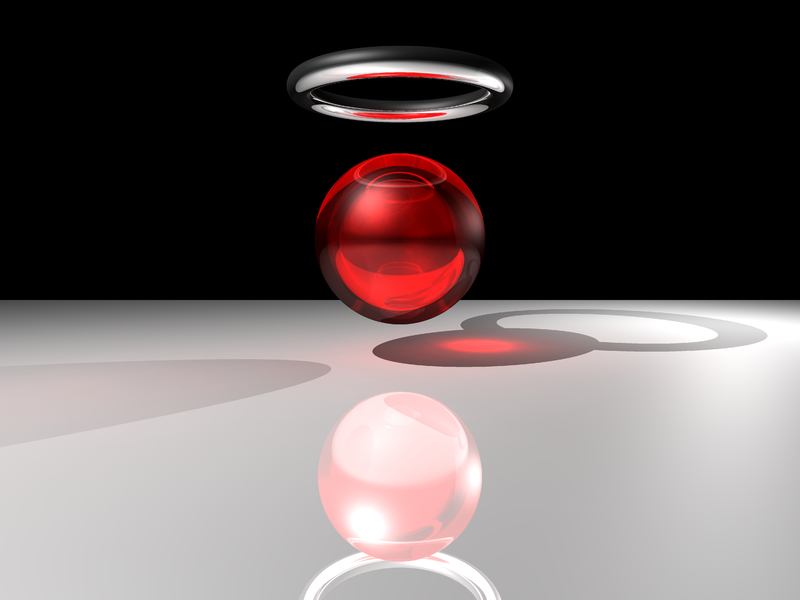
\includegraphics[width=8cm]{OGL_intro/raytracing.png}
    \caption{광선 추적법을 적용한 결과}
    \label{fig:OGL_intro:raytracing}
\end{figure}

\subsubsection{1990 년대}

컴퓨터 그래픽스를 처리하는 전담 하드웨어가 개인용 컴퓨터에 표준적으로 설치되기 시작했으며, 이러한 하드웨어에 힘입어 실시간 그래픽스 분야가 획기적인 발전을 이루게 된다. 90 년대에 들어와서 실시간 그래픽스를 처리하는 데에 있어 매우 중요한 OpenGL API(application programming interface)가 완성되며, 개인용 컴퓨터에서도 텍스처 매핑, 블렌딩(blending)이 손쉽게 이루어지게 되며, 다양한 종류의 버퍼(buffer) 활용 기술도 적용된다.
이 무렵 컴퓨터 그래픽스를 이용하여 제작된 애니메이션 작품들이 대단한 성공을 거두게 되어 관련 산업의 발전을 촉진하게 된다. 
이 당시의 컴퓨터 그래픽스에 대한 연구와 상업적 활용은 실리콘 그래픽스(SGI)의 워크스테이션을 통해 구현되는 경우가 많았으며, 이 회사에서 만든 OpenGL이 그래픽 프로그래밍의 표준적 API로 자리잡게 된다. 그림 \ref{fig:OGL_intro:SGI}는 실리콘 그래픽스에서 판매한 O2, 인디고(Indigo), 옥테인(Octane) 등의 그래픽 워크스테이션 제품들이다.

\begin{figure}[h!]
  \centering
    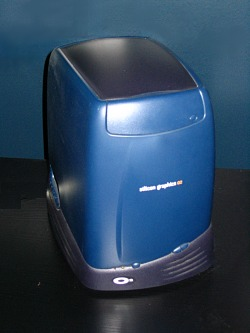
\includegraphics[height=5cm]{OGL_intro/SGI_O2.jpg}
    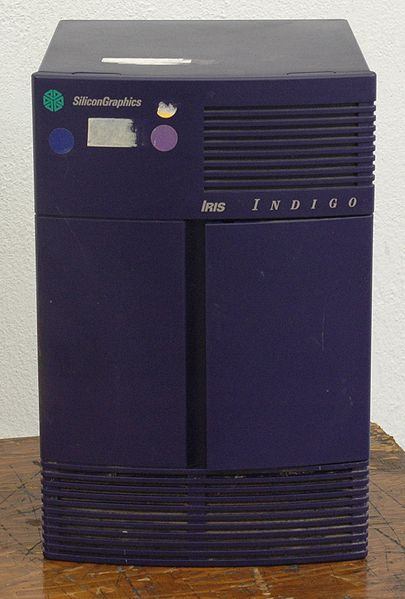
\includegraphics[height=5cm]{OGL_intro/SGI_Indigo.jpg}
    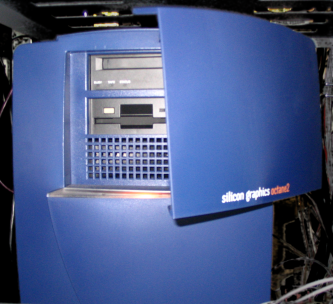
\includegraphics[height=5cm]{OGL_intro/SGI_Octane.png}
    \caption{실리콘 그래픽스에서 출시한 그래픽 워크스테이션}
    \label{fig:OGL_intro:SGI}
\end{figure}

\subsubsection{2000 년 이후}

극사실적 그래픽 표현 기술이 그림 \ref{fig:OGL_intro:photorealisticTeapot}과 같이 실사와 그래픽스 표현을 구분할 수 없는 수준까지 이르게 된다. 실시간 그래픽스 분야에서는 NVIDIA, ATI의 경쟁 구도로 매우 빠른 속도의 하드웨어 성능 개선이 이루어지며, 게임이 시장의 중요한 동력으로 자리잡게 된다. 그래픽처리 장치는 프로그램 가능한 형태로 바뀌었으며, 이를 활용한 렌더링 뿐만 아니라, GPU의 병렬처리 능력을 활용한 효율적인 애니메이션이나 계산 등도 이루어지게 된다.

\begin{figure}[h!]
  \centering
    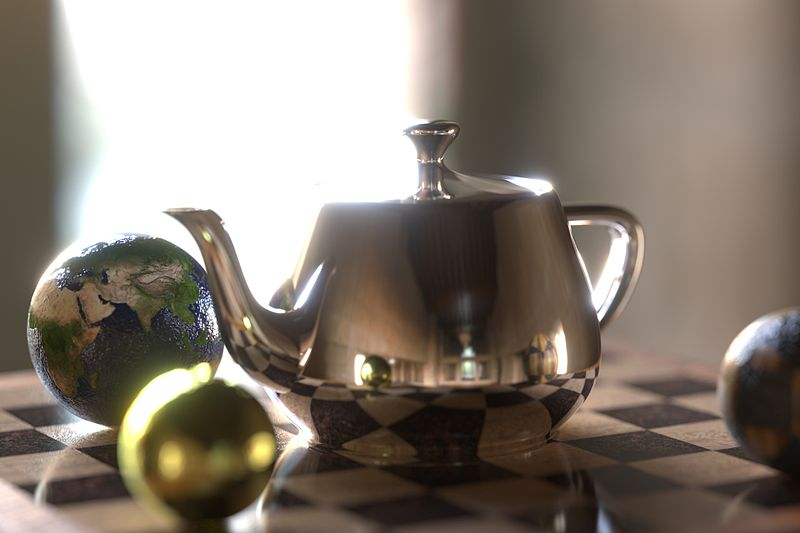
\includegraphics[width=8cm]{OGL_intro/photorealisticTeapot.jpg}
    \caption{사실적 렌더링의 예}
    \label{fig:OGL_intro:photorealisticTeapot}
\end{figure}

\section{3차원 공간의 표현과 영상 생성의 기본 개념}

이 절에서는 가상의 3차원 공간에 표현된 환경을 2차원 영상 이미지로 만들어 내는 일과 관련된 기본적인 개념을 설명할 것이다. 이미지를 만들어내는 데에는 기본적으로 다음과 같은 세 가지 물리적 요소가 고려되어야 한다.

\begin{itemize}
\item 광원(Light)
\item 색(Color)
\item 인지(Perception)
\end{itemize}

컴퓨터 그래픽스를 통해 이미지를 생성할 때 실제 광학 시스템의 모델을 차용하여 카메라 모델을 만드는 것을 합성 카메라 모델(synthetic camera model)이라고 부른다. 

컴퓨터 그래픽스에서 차용하는 물리적 영상 시스템의 예로는 다음과 같은 것들이 존재한다.
카메라, 현미경, 망원경, 인간 시각
이러한 광학 시스템에서 영상이 맺히는 방식을 흉내내어 가상의 카메라를 만드는 것이 바라 합성 카메라 모델이다.
영상 생성에 있어 필요한 최소한의 요소 객체는 아래에 나타나 있는 것과 같은 객체, 관측자, 광원이다.
영상 생성의 핵심은 광원에서 나온 빛이 객체에 어떻게 반사되어 관측자에게 도달하는가이다. 
이때 관측자, 광원, 카메라는 상호 독립적인 객체로서 서로의 속성에 영향을 미치지 않는다. 이제 이들 각각에 대해 살펴보도록 하자.

\subsubsection{광원(Light Source)}
광원은 빛을 발생시키는 객체, 혹은 지점이다. 빛이란 전자기파의 일부로 우리 눈이 반응하는 스펙트럼 영역을 의미한다. 빛과 색에 대해서는 다시 다룰 것인데, 간략히 설명하면 390nm~720nm 정도의 범위의 전자기파로서 파장인 긴 쪽은 붉은색 짧은 쪽은 자색을 띠게 된다.
광원이 중요한 이유는 우리가 영상으로 담아내는 내용은 빛이 객체와 반응하여 관측자에게 도달한 결과이기 때문이다. 사진이나 우리 눈 모두 이런 빛을 감지하는 도구라고 할 수 있다. 


\subsubsection{광선 추적 기법(Ray Tracing Method)}

\index{광선 추적법}
영상이 빛을 담아내는 것이라면 가장 간단한 접근법은 그림 \ref{fig:OGL_intro:raytracingConcept}와 같이 광원에서 나온 빛을 추적하여 객체에 충돌하고 반사하는 과정을 계산한 뒤에 관측자의 영상 시스템에 도달하는 결과를 알아내는 것이다. 
이 방법의 단점은 관측자에게 도달하기 전에 빛이 객체와 매우 많은 상호작용을 하게될 수 있으며, 때론 무한히 반사할 수 있어 완벽히 추적하는 것이 불가능하다는 것이다.

\begin{figure}[h!]
  \centering
    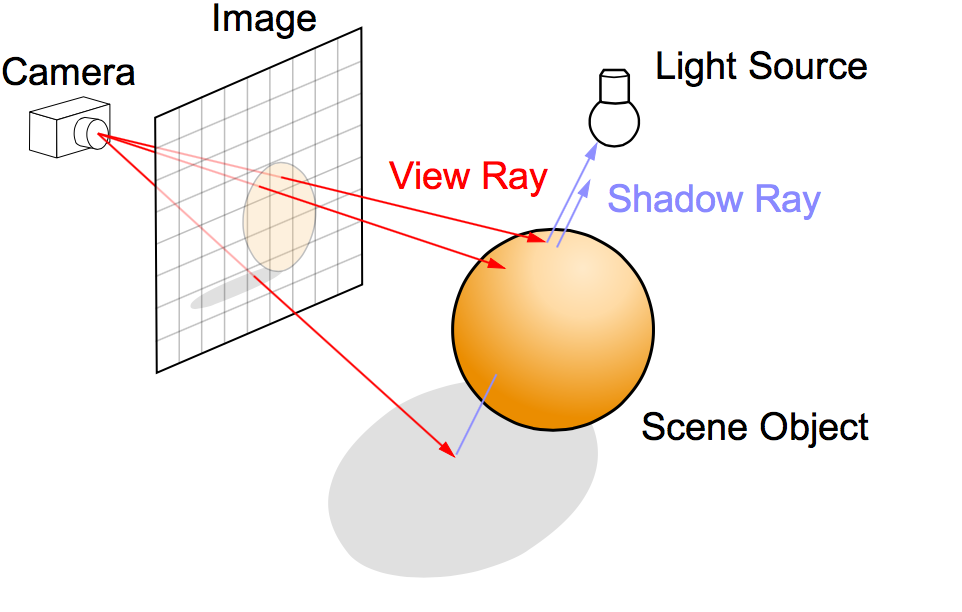
\includegraphics[height=5cm]{OGL_intro/raytracingConcept.png}
    \caption{광선 추적법의 개념}
    \label{fig:OGL_intro:raytracingConcept}
\end{figure}

\subsubsection{바늘구멍 카메라(Pinhole Camera)}

\index{바늘 구멍 카메라}\index{pin hole camera}
바늘구멍 카메라는 빛이 차단된 통에 작은 구멍을 내고 이 구멍을 통해 들어온 빛이 반대편 벽에 상을 맺게 하는 것이다. 그림 \ref{fig:OGL_intro:pinhole}에서 볼 수 있는 바와 같이  $(x,y,z)$의 위치에 있는 기하객체는 원점에 있는 구멍을 통과하여 $z=-d$의 평면에 상을 맺게 되는데, 상의 위치 $(x_p, y_p, z_p)$는 다음과 같이 쉽게 계산할 수 있다. 이 계산이 간단한 원근 투영법의 기본적 원리이다.



\begin{eqnarray}
\left ( x_p = - \frac{x d}{z} , y_p = - \frac{yd}{z}, z_p = -d \right )
\end{eqnarray}

\begin{figure}[h!]
  \centering
    \begin{tikzpicture} [scale=3]
      \draw  (0,0) -- (1,0) -- (1,0.5) -- (0,0.5) -- cycle;
	\draw (0.5, 0.25) -- (1.5, 0.25) -- (1.5, 0.75) -- (0.5, 0.75) -- cycle;
	\draw (0.5, 0.75) -- (0,0.5);
	\draw (0.5, 0.25) -- (0,0);
	\draw (1.5,0.75) -- (1.0,0.5);
	\draw (1.5, 0.25) -- (1.0,0);
	\draw [<->] (0,-0.25) -- (1,-0.25);
	\draw (0.5,-0.3) node {$d$};
	\draw (1.25, 0.375) circle (0.04);
	\draw [->] (1.25, 0.375) -- (2.0, 0.375);
	\draw [->] (1.25, 0.375) -- (1.25, 1.0);
	\draw [->] (1.25, 0.375) -- (1.75, 0.65);
	\draw (0.20, 0.17) -- (1.75, 0.5);
	\draw [fill] (0.2,0.17) circle [radius=0.02];
	\draw [fill] (1.75,0.5) circle [radius=0.02];
	\draw (0.0, 0.27) node (xp) {$(x_p, y_p, z_p)$};
	\draw (2.0, 0.5) node (xp) {$(x, y, z)$};
	\draw (2.0, 0.3) node {$x$};
	\draw (1.4, 1.0) node {$y$};
	\draw (1.75, 0.75) node {$z$};
   \end{tikzpicture}
    \caption{바늘구멍 카메라의 원리}
    \label{fig:OGL_intro:pinhole}
\end{figure}

\subsubsection{합성 카메라 모델(Synthetic Camera Model)}

\index{카메라!합성 카메라 모델}
합성 카메라 모델은 카메라와 같은 가상의 광학 시스템을 구성하여 가상 객체를 담아내는 것이다. 바늘구멍 카메라와 같이 구멍을 통과하는 것이 아니라, 구멍을 통과하기 전에 적절한 거리 d 만큼 앞에 구멍을 향해 진행하는 빛을 잡아낼 수 있는 평면을 두게 되면, 구멍 뒤의 평면에 상이 거꾸로 맺히는 것과 달리 원래의 모양대로 상이 맺히게 된다. 합성 카메라 모델에서는 일반적으로 이러한 방식을 사용하고 있다. 이때 빛이 모이는 곳, 혹은 카메라의 위치를 원점으로 보고 카메라가 $z$ 축을 향하고 있다면 상이 맺히는 곳은 다음과 같이 계산할 수 있다.


\begin{eqnarray}
\left ( x_p = \frac{x d}{z} , y_p = \frac{yd}{z}, z_p = d \right )
\end{eqnarray}

이러한 합성 카메라 모델은 객체와 관측자, 광원을 분리하여 다룰 수 있게 하며, 객체, 광원, 카메라의 속성을 설정하는 간단한 소프트웨어 API로 모델을 만들 수 있다. 또한 이 방식은 고속으로 처리가능한 하드웨어 구현이 용이하다는 장점도 가진다.

\subsubsection{전역조명과 지역조명(Global Illumination and Local Illumination)}

\index{전역조명}\index{지역조명}
\index{global illumination}\index{local illumination}
실제 현실의 물체와 같은 색상이나 음영을 계산하기 위해서는 각각의 가상 물체를 독립적으로 다루어서는 안된다. 일부 객체는 다른 객체에 의해 빛이 가려져 있을 수도 있고, 빛이 반사되어 다른 객체로 가기도 하며, 어떤 객체는 빛을 통과시킬 수도 있다. 이러한 것들을 고려하려면 하나의 객체만을 놓고 광원과의 관계를 고려하여 색을 결정하는 것이 아니라 모든 객체를 동시에 고려하여 색을 결정하여야 한다. 이런 방식을 전역 조명 방식이라 하는데, 실시간 환경에서 구현하기가 쉽지 않다. 따라서 OpenGL이나 DirectX와 같은 실시간 그래픽스 라이브러리에서는 지역조명, 즉 다른 객체가 모두 존재하지 않는다고 가정하고 객체의 각 면과 광원의 관계만 고려하여 색상을 결정하는 방식을 사용한다.
앞서 언급한 광선 추적 기법 역시 많은 시간을 요구하는 방식이다. 따라서 이 방식이 좋은 영상을 생성할 수 있다할지라도 실시간 환경에서는 일반적으로 적용되지 않는다. 
그림 \ref{fig:OGL_intro:localVsGlobalIllumination}은 지역 조명과 전역 조명 모델이 어떠한 차이를 보이는지 비교하고 있다.




\begin{figure}[h!]
  \centering
	\begin{tabular}{cc}
	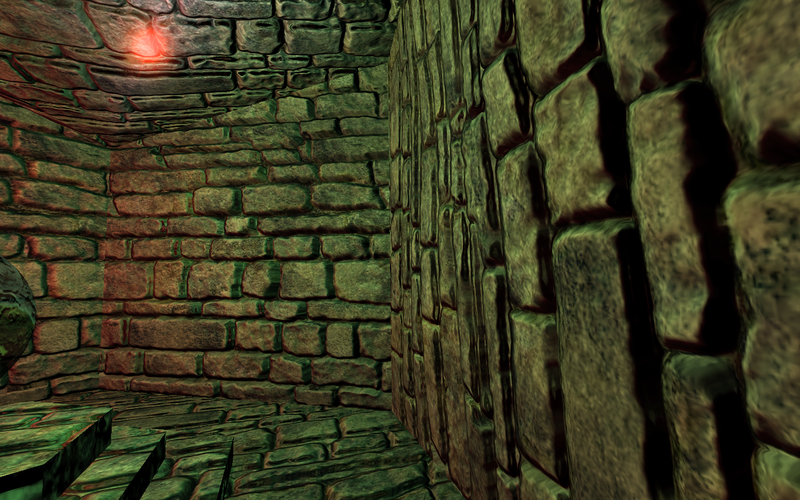
\includegraphics[height=4cm]{OGL_intro/realtimeEx.png} &    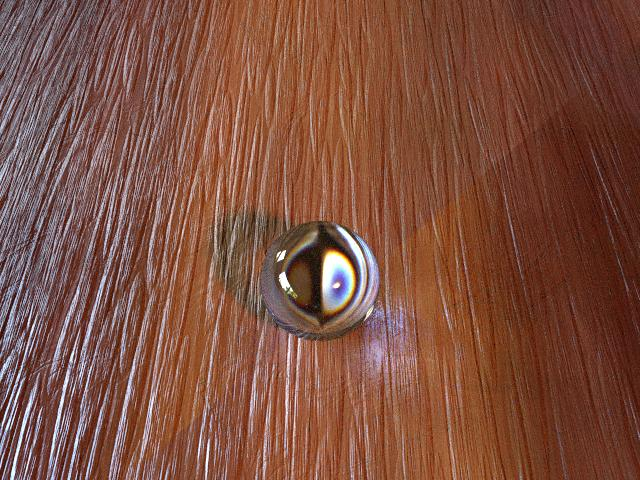
\includegraphics[height=4cm]{OGL_intro/offlineEx.jpg} \\
	(a) 지역조명 & (b) 전역조명
	\end{tabular}
    \caption{지역조명과 전역조명을 적용한 렌더링 결과의 비교}
    \label{fig:OGL_intro:localVsGlobalIllumination}
\end{figure}


